%% BioMed_Central_Tex_Template_v1.06
%%                                      %
%  bmc_article.tex            ver: 1.06 %
%                                       %

%%IMPORTANT: do not delete the first line of this template
%%It must be present to enable the BMC Submission system to
%%recognise this template!!

%%%%%%%%%%%%%%%%%%%%%%%%%%%%%%%%%%%%%%%%%
%%                                     %%
%%  LaTeX template for BioMed Central  %%
%%     journal article submissions     %%
%%                                     %%
%%          <8 June 2012>              %%
%%                                     %%
%%                                     %%
%%%%%%%%%%%%%%%%%%%%%%%%%%%%%%%%%%%%%%%%%


%%%%%%%%%%%%%%%%%%%%%%%%%%%%%%%%%%%%%%%%%%%%%%%%%%%%%%%%%%%%%%%%%%%%%
%%                                                                 %%
%% For instructions on how to fill out this Tex template           %%
%% document please refer to Readme.html and the instructions for   %%
%% authors page on the biomed central website                      %%
%% http://www.biomedcentral.com/info/authors/                      %%
%%                                                                 %%
%% Please do not use \input{...} to include other tex files.       %%
%% Submit your LaTeX manuscript as one .tex document.              %%
%%                                                                 %%
%% All additional figures and files should be attached             %%
%% separately and not embedded in the \TeX\ document itself.       %%
%%                                                                 %%
%% BioMed Central currently use the MikTex distribution of         %%
%% TeX for Windows) of TeX and LaTeX.  This is available from      %%
%% http://www.miktex.org                                           %%
%%                                                                 %%
%%%%%%%%%%%%%%%%%%%%%%%%%%%%%%%%%%%%%%%%%%%%%%%%%%%%%%%%%%%%%%%%%%%%%

%%% additional documentclass options:
%  [doublespacing]
%  [linenumbers]   - put the line numbers on margins

%%% loading packages, author definitions

%\documentclass[twocolumn]{bmcart}% uncomment this for twocolumn layout and comment line below
\documentclass{bmcart}

%%% Load packages
\usepackage{amsthm,amsmath}
%\RequirePackage{natbib}
%\RequirePackage[authoryear]{natbib}% uncomment this for author-year bibliography
%\RequirePackage{hyperref}
% \usepackage[utf8]{inputenc} %unicode support
%\usepackage[applemac]{inputenc} %applemac support if unicode package fails
%\usepackage[latin1]{inputenc} %UNIX support if unicode package fails
\usepackage{graphicx}
\usepackage{cite}
\usepackage{xcolor}
\usepackage{courier}



%%%%%%%%%%%%%%%%%%%%%%%%%%%%From Notebook%%%%%%%%%%%%%%%%%%%%%%%%%%

    \usepackage{graphicx} % Used to insert images
    \usepackage{adjustbox} % Used to constrain images to a maximum size
    \usepackage{color} % Allow colors to be defined
    \usepackage{enumerate} % Needed for markdown enumerations to work
    % \usepackage{geometry} % Used to adjust the document margins
    \usepackage{amsmath} % Equations
    \usepackage{amssymb} % Equations
    \usepackage{eurosym} % defines \euro
    \usepackage[mathletters]{ucs} % Extended unicode (utf-8) support
    \usepackage[utf8x]{inputenc} % Allow utf-8 characters in the tex document
    \usepackage{fancyvrb} % verbatim replacement that allows latex
    \usepackage{grffile} % extends the file name processing of package graphics
                         % to support a larger range
    % The hyperref package gives us a pdf with properly built
    % internal navigation ('pdf bookmarks' for the table of contents,
    % internal cross-reference links, web links for URLs, etc.)
    \usepackage{hyperref}
    \usepackage{longtable} % longtable support required by pandoc >1.10
    \usepackage{booktabs}  % table support for pandoc > 1.12.2
    \usepackage{ulem} % ulem is needed to support strikethroughs (\sout)
    \usepackage{listings} % code blocks




    \definecolor{orange}{cmyk}{0,0.4,0.8,0.2}
    \definecolor{darkorange}{rgb}{.71,0.21,0.01}
    \definecolor{darkgreen}{rgb}{.12,.54,.11}
    \definecolor{myteal}{rgb}{.26, .44, .56}
    \definecolor{gray}{gray}{0.45}
    \definecolor{lightgray}{gray}{.95}
    \definecolor{mediumgray}{gray}{.8}
    \definecolor{inputbackground}{rgb}{.95, .95, .85}
    \definecolor{outputbackground}{rgb}{.95, .95, .95}
    \definecolor{traceback}{rgb}{1, .95, .95}
    % ansi colors
    \definecolor{red}{rgb}{.6,0,0}
    \definecolor{green}{rgb}{0,.65,0}
    \definecolor{brown}{rgb}{0.6,0.6,0}
    \definecolor{blue}{rgb}{0,.145,.698}
    \definecolor{purple}{rgb}{.698,.145,.698}
    \definecolor{cyan}{rgb}{0,.698,.698}
    \definecolor{lightgray}{gray}{0.5}

    % bright ansi colors
    \definecolor{darkgray}{gray}{0.25}
    \definecolor{lightred}{rgb}{1.0,0.39,0.28}
    \definecolor{lightgreen}{rgb}{0.48,0.99,0.0}
    \definecolor{lightblue}{rgb}{0.53,0.81,0.92}
    \definecolor{lightpurple}{rgb}{0.87,0.63,0.87}
    \definecolor{lightcyan}{rgb}{0.5,1.0,0.83}

    % commands and environments needed by pandoc snippets
    % extracted from the output of `pandoc -s`
    \providecommand{\tightlist}{%
      \setlength{\itemsep}{0pt}\setlength{\parskip}{0pt}}
    \DefineVerbatimEnvironment{Highlighting}{Verbatim}{commandchars=\\\{\}}
    % Add ',fontsize=\small' for more characters per line
    \newenvironment{Shaded}{}{}
    \newcommand{\KeywordTok}[1]{\textcolor[rgb]{0.00,0.44,0.13}{\textbf{{#1}}}}
    \newcommand{\DataTypeTok}[1]{\textcolor[rgb]{0.56,0.13,0.00}{{#1}}}
    \newcommand{\DecValTok}[1]{\textcolor[rgb]{0.25,0.63,0.44}{{#1}}}
    \newcommand{\BaseNTok}[1]{\textcolor[rgb]{0.25,0.63,0.44}{{#1}}}
    \newcommand{\FloatTok}[1]{\textcolor[rgb]{0.25,0.63,0.44}{{#1}}}
    \newcommand{\CharTok}[1]{\textcolor[rgb]{0.25,0.44,0.63}{{#1}}}
    \newcommand{\StringTok}[1]{\textcolor[rgb]{0.25,0.44,0.63}{{#1}}}
    \newcommand{\CommentTok}[1]{\textcolor[rgb]{0.38,0.63,0.69}{\textit{{#1}}}}
    \newcommand{\OtherTok}[1]{\textcolor[rgb]{0.00,0.44,0.13}{{#1}}}
    \newcommand{\AlertTok}[1]{\textcolor[rgb]{1.00,0.00,0.00}{\textbf{{#1}}}}
    \newcommand{\FunctionTok}[1]{\textcolor[rgb]{0.02,0.16,0.49}{{#1}}}
    \newcommand{\RegionMarkerTok}[1]{{#1}}
    \newcommand{\ErrorTok}[1]{\textcolor[rgb]{1.00,0.00,0.00}{\textbf{{#1}}}}
    \newcommand{\NormalTok}[1]{{#1}}

    % Additional commands for more recent versions of Pandoc
    \newcommand{\ConstantTok}[1]{\textcolor[rgb]{0.53,0.00,0.00}{{#1}}}
    \newcommand{\SpecialCharTok}[1]{\textcolor[rgb]{0.25,0.44,0.63}{{#1}}}
    \newcommand{\VerbatimStringTok}[1]{\textcolor[rgb]{0.25,0.44,0.63}{{#1}}}
    \newcommand{\SpecialStringTok}[1]{\textcolor[rgb]{0.73,0.40,0.53}{{#1}}}
    \newcommand{\ImportTok}[1]{{#1}}
    \newcommand{\DocumentationTok}[1]{\textcolor[rgb]{0.73,0.13,0.13}{\textit{{#1}}}}
    \newcommand{\AnnotationTok}[1]{\textcolor[rgb]{0.38,0.63,0.69}{\textbf{\textit{{#1}}}}}
    \newcommand{\CommentVarTok}[1]{\textcolor[rgb]{0.38,0.63,0.69}{\textbf{\textit{{#1}}}}}
    \newcommand{\VariableTok}[1]{\textcolor[rgb]{0.10,0.09,0.49}{{#1}}}
    \newcommand{\ControlFlowTok}[1]{\textcolor[rgb]{0.00,0.44,0.13}{\textbf{{#1}}}}
    \newcommand{\OperatorTok}[1]{\textcolor[rgb]{0.40,0.40,0.40}{{#1}}}
    \newcommand{\BuiltInTok}[1]{{#1}}
    \newcommand{\ExtensionTok}[1]{{#1}}
    \newcommand{\PreprocessorTok}[1]{\textcolor[rgb]{0.74,0.48,0.00}{{#1}}}
    \newcommand{\AttributeTok}[1]{\textcolor[rgb]{0.49,0.56,0.16}{{#1}}}
    \newcommand{\InformationTok}[1]{\textcolor[rgb]{0.38,0.63,0.69}{\textbf{\textit{{#1}}}}}
    \newcommand{\WarningTok}[1]{\textcolor[rgb]{0.38,0.63,0.69}{\textbf{\textit{{#1}}}}}


    % Define a nice break command that doesn't care if a line doesn't already
    % exist.
    \def\br{\hspace*{\fill} \\* }
    % Math Jax compatability definitions
    \def\gt{>}
    \def\lt{<}

\makeatletter
\def\PY@reset{\let\PY@it=\relax \let\PY@bf=\relax%
    \let\PY@ul=\relax \let\PY@tc=\relax%
    \let\PY@bc=\relax \let\PY@ff=\relax}
\def\PY@tok#1{\csname PY@tok@#1\endcsname}
\def\PY@toks#1+{\ifx\relax#1\empty\else%
    \PY@tok{#1}\expandafter\PY@toks\fi}
\def\PY@do#1{\PY@bc{\PY@tc{\PY@ul{%
    \PY@it{\PY@bf{\PY@ff{#1}}}}}}}
\def\PY#1#2{\PY@reset\PY@toks#1+\relax+\PY@do{#2}}

\expandafter\def\csname PY@tok@gd\endcsname{\def\PY@tc##1{\textcolor[rgb]{0.63,0.00,0.00}{##1}}}
\expandafter\def\csname PY@tok@gu\endcsname{\let\PY@bf=\textbf\def\PY@tc##1{\textcolor[rgb]{0.50,0.00,0.50}{##1}}}
\expandafter\def\csname PY@tok@gt\endcsname{\def\PY@tc##1{\textcolor[rgb]{0.00,0.27,0.87}{##1}}}
\expandafter\def\csname PY@tok@gs\endcsname{\let\PY@bf=\textbf}
\expandafter\def\csname PY@tok@gr\endcsname{\def\PY@tc##1{\textcolor[rgb]{1.00,0.00,0.00}{##1}}}
\expandafter\def\csname PY@tok@cm\endcsname{\let\PY@it=\textit\def\PY@tc##1{\textcolor[rgb]{0.25,0.50,0.50}{##1}}}
\expandafter\def\csname PY@tok@vg\endcsname{\def\PY@tc##1{\textcolor[rgb]{0.10,0.09,0.49}{##1}}}
\expandafter\def\csname PY@tok@vi\endcsname{\def\PY@tc##1{\textcolor[rgb]{0.10,0.09,0.49}{##1}}}
\expandafter\def\csname PY@tok@mh\endcsname{\def\PY@tc##1{\textcolor[rgb]{0.40,0.40,0.40}{##1}}}
\expandafter\def\csname PY@tok@cs\endcsname{\let\PY@it=\textit\def\PY@tc##1{\textcolor[rgb]{0.25,0.50,0.50}{##1}}}
\expandafter\def\csname PY@tok@ge\endcsname{\let\PY@it=\textit}
\expandafter\def\csname PY@tok@vc\endcsname{\def\PY@tc##1{\textcolor[rgb]{0.10,0.09,0.49}{##1}}}
\expandafter\def\csname PY@tok@il\endcsname{\def\PY@tc##1{\textcolor[rgb]{0.40,0.40,0.40}{##1}}}
\expandafter\def\csname PY@tok@go\endcsname{\def\PY@tc##1{\textcolor[rgb]{0.53,0.53,0.53}{##1}}}
\expandafter\def\csname PY@tok@cp\endcsname{\def\PY@tc##1{\textcolor[rgb]{0.74,0.48,0.00}{##1}}}
\expandafter\def\csname PY@tok@gi\endcsname{\def\PY@tc##1{\textcolor[rgb]{0.00,0.63,0.00}{##1}}}
\expandafter\def\csname PY@tok@gh\endcsname{\let\PY@bf=\textbf\def\PY@tc##1{\textcolor[rgb]{0.00,0.00,0.50}{##1}}}
\expandafter\def\csname PY@tok@ni\endcsname{\let\PY@bf=\textbf\def\PY@tc##1{\textcolor[rgb]{0.60,0.60,0.60}{##1}}}
\expandafter\def\csname PY@tok@nl\endcsname{\def\PY@tc##1{\textcolor[rgb]{0.63,0.63,0.00}{##1}}}
\expandafter\def\csname PY@tok@nn\endcsname{\let\PY@bf=\textbf\def\PY@tc##1{\textcolor[rgb]{0.00,0.00,1.00}{##1}}}
\expandafter\def\csname PY@tok@no\endcsname{\def\PY@tc##1{\textcolor[rgb]{0.53,0.00,0.00}{##1}}}
\expandafter\def\csname PY@tok@na\endcsname{\def\PY@tc##1{\textcolor[rgb]{0.49,0.56,0.16}{##1}}}
\expandafter\def\csname PY@tok@nb\endcsname{\def\PY@tc##1{\textcolor[rgb]{0.00,0.50,0.00}{##1}}}
\expandafter\def\csname PY@tok@nc\endcsname{\let\PY@bf=\textbf\def\PY@tc##1{\textcolor[rgb]{0.00,0.00,1.00}{##1}}}
\expandafter\def\csname PY@tok@nd\endcsname{\def\PY@tc##1{\textcolor[rgb]{0.67,0.13,1.00}{##1}}}
\expandafter\def\csname PY@tok@ne\endcsname{\let\PY@bf=\textbf\def\PY@tc##1{\textcolor[rgb]{0.82,0.25,0.23}{##1}}}
\expandafter\def\csname PY@tok@nf\endcsname{\def\PY@tc##1{\textcolor[rgb]{0.00,0.00,1.00}{##1}}}
\expandafter\def\csname PY@tok@si\endcsname{\let\PY@bf=\textbf\def\PY@tc##1{\textcolor[rgb]{0.73,0.40,0.53}{##1}}}
\expandafter\def\csname PY@tok@s2\endcsname{\def\PY@tc##1{\textcolor[rgb]{0.73,0.13,0.13}{##1}}}
\expandafter\def\csname PY@tok@nt\endcsname{\let\PY@bf=\textbf\def\PY@tc##1{\textcolor[rgb]{0.00,0.50,0.00}{##1}}}
\expandafter\def\csname PY@tok@nv\endcsname{\def\PY@tc##1{\textcolor[rgb]{0.10,0.09,0.49}{##1}}}
\expandafter\def\csname PY@tok@s1\endcsname{\def\PY@tc##1{\textcolor[rgb]{0.73,0.13,0.13}{##1}}}
\expandafter\def\csname PY@tok@ch\endcsname{\let\PY@it=\textit\def\PY@tc##1{\textcolor[rgb]{0.25,0.50,0.50}{##1}}}
\expandafter\def\csname PY@tok@m\endcsname{\def\PY@tc##1{\textcolor[rgb]{0.40,0.40,0.40}{##1}}}
\expandafter\def\csname PY@tok@gp\endcsname{\let\PY@bf=\textbf\def\PY@tc##1{\textcolor[rgb]{0.00,0.00,0.50}{##1}}}
\expandafter\def\csname PY@tok@sh\endcsname{\def\PY@tc##1{\textcolor[rgb]{0.73,0.13,0.13}{##1}}}
\expandafter\def\csname PY@tok@ow\endcsname{\let\PY@bf=\textbf\def\PY@tc##1{\textcolor[rgb]{0.67,0.13,1.00}{##1}}}
\expandafter\def\csname PY@tok@sx\endcsname{\def\PY@tc##1{\textcolor[rgb]{0.00,0.50,0.00}{##1}}}
\expandafter\def\csname PY@tok@bp\endcsname{\def\PY@tc##1{\textcolor[rgb]{0.00,0.50,0.00}{##1}}}
\expandafter\def\csname PY@tok@c1\endcsname{\let\PY@it=\textit\def\PY@tc##1{\textcolor[rgb]{0.25,0.50,0.50}{##1}}}
\expandafter\def\csname PY@tok@o\endcsname{\def\PY@tc##1{\textcolor[rgb]{0.40,0.40,0.40}{##1}}}
\expandafter\def\csname PY@tok@kc\endcsname{\let\PY@bf=\textbf\def\PY@tc##1{\textcolor[rgb]{0.00,0.50,0.00}{##1}}}
\expandafter\def\csname PY@tok@c\endcsname{\let\PY@it=\textit\def\PY@tc##1{\textcolor[rgb]{0.25,0.50,0.50}{##1}}}
\expandafter\def\csname PY@tok@mf\endcsname{\def\PY@tc##1{\textcolor[rgb]{0.40,0.40,0.40}{##1}}}
\expandafter\def\csname PY@tok@err\endcsname{\def\PY@bc##1{\setlength{\fboxsep}{0pt}\fcolorbox[rgb]{1.00,0.00,0.00}{1,1,1}{\strut ##1}}}
\expandafter\def\csname PY@tok@mb\endcsname{\def\PY@tc##1{\textcolor[rgb]{0.40,0.40,0.40}{##1}}}
\expandafter\def\csname PY@tok@ss\endcsname{\def\PY@tc##1{\textcolor[rgb]{0.10,0.09,0.49}{##1}}}
\expandafter\def\csname PY@tok@sr\endcsname{\def\PY@tc##1{\textcolor[rgb]{0.73,0.40,0.53}{##1}}}
\expandafter\def\csname PY@tok@mo\endcsname{\def\PY@tc##1{\textcolor[rgb]{0.40,0.40,0.40}{##1}}}
\expandafter\def\csname PY@tok@kd\endcsname{\let\PY@bf=\textbf\def\PY@tc##1{\textcolor[rgb]{0.00,0.50,0.00}{##1}}}
\expandafter\def\csname PY@tok@mi\endcsname{\def\PY@tc##1{\textcolor[rgb]{0.40,0.40,0.40}{##1}}}
\expandafter\def\csname PY@tok@kn\endcsname{\let\PY@bf=\textbf\def\PY@tc##1{\textcolor[rgb]{0.00,0.50,0.00}{##1}}}
\expandafter\def\csname PY@tok@cpf\endcsname{\let\PY@it=\textit\def\PY@tc##1{\textcolor[rgb]{0.25,0.50,0.50}{##1}}}
\expandafter\def\csname PY@tok@kr\endcsname{\let\PY@bf=\textbf\def\PY@tc##1{\textcolor[rgb]{0.00,0.50,0.00}{##1}}}
\expandafter\def\csname PY@tok@s\endcsname{\def\PY@tc##1{\textcolor[rgb]{0.73,0.13,0.13}{##1}}}
\expandafter\def\csname PY@tok@kp\endcsname{\def\PY@tc##1{\textcolor[rgb]{0.00,0.50,0.00}{##1}}}
\expandafter\def\csname PY@tok@w\endcsname{\def\PY@tc##1{\textcolor[rgb]{0.73,0.73,0.73}{##1}}}
\expandafter\def\csname PY@tok@kt\endcsname{\def\PY@tc##1{\textcolor[rgb]{0.69,0.00,0.25}{##1}}}
\expandafter\def\csname PY@tok@sc\endcsname{\def\PY@tc##1{\textcolor[rgb]{0.73,0.13,0.13}{##1}}}
\expandafter\def\csname PY@tok@sb\endcsname{\def\PY@tc##1{\textcolor[rgb]{0.73,0.13,0.13}{##1}}}
\expandafter\def\csname PY@tok@k\endcsname{\let\PY@bf=\textbf\def\PY@tc##1{\textcolor[rgb]{0.00,0.50,0.00}{##1}}}
\expandafter\def\csname PY@tok@se\endcsname{\let\PY@bf=\textbf\def\PY@tc##1{\textcolor[rgb]{0.73,0.40,0.13}{##1}}}
\expandafter\def\csname PY@tok@sd\endcsname{\let\PY@it=\textit\def\PY@tc##1{\textcolor[rgb]{0.73,0.13,0.13}{##1}}}

\def\PYZbs{\char`\\}
\def\PYZus{\char`\_}
\def\PYZob{\char`\{}
\def\PYZcb{\char`\}}
\def\PYZca{\char`\^}
\def\PYZam{\char`\&}
\def\PYZlt{\char`\<}
\def\PYZgt{\char`\>}
\def\PYZsh{\char`\#}
\def\PYZpc{\char`\%}
\def\PYZdl{\char`\$}
\def\PYZhy{\char`\-}
\def\PYZsq{\char`\'}
\def\PYZdq{\char`\"}
\def\PYZti{\char`\~}
% for compatibility with earlier versions
\def\PYZat{@}
\def\PYZlb{[}
\def\PYZrb{]}
\makeatother


    % Exact colors from NB
    \definecolor{incolor}{rgb}{0.0, 0.0, 0.5}
    \definecolor{outcolor}{rgb}{0.545, 0.0, 0.0}

  \definecolor{codegreen}{rgb}{0,0.6,0}
  \definecolor{codegray}{rgb}{0.5,0.5,0.5}
  \definecolor{codepurple}{rgb}{0.58,0,0.82}
  \definecolor{backcolour}{rgb}{0.95,0.95,0.92}
  \definecolor{outcolor}{rgb}{0.7,0.7,0.7}

% Python style for highlighting
\lstdefinestyle{input}{
    backgroundcolor=\color{backcolour},
    commentstyle=\color{codegreen},
    keywordstyle=\color{codegreen},
    numberstyle=\tiny\color{white},
    basicstyle=\ttfamily\linespread{1.2}\small,
    breakatwhitespace=false,
    breaklines=true,
    captionpos=b,
    keepspaces=true,
    numbers=left,
    numbersep=5pt,
    showspaces=false,
    showstringspaces=false,
    showtabs=false,
    tabsize=2,
    stringstyle=\color{red},
    language={Python},
    emph={__future__, pymks, datasets, tools, sklearn, cross_validation, grid_search, bases},
    emphstyle=\color{blue},
    belowskip=0.3em,
    aboveskip=1em,
%     otherkeywords={ as },
}
%
% Python style for highlighting
\lstdefinestyle{output}{
	style=input,
    backgroundcolor=\color{white},
	frame=single,
    rulecolor=\color{outcolor},
    aboveskip=0.3em,
    belowskip=1em,
}

\newcommand{\fimage}
{\fcolorbox{outcolor}{white}}
{}

\lstnewenvironment{_output}
{\lstset{style=output}}
{}

\lstnewenvironment{_input}
{\lstset{style=input}}
{}



% \lstset{style=mystyle,
%     % Custom highlighting style
%         language=python}

    % Prevent overflowing lines due to hard-to-break entities
    \sloppy
    % Setup hyperref package
    % \hypersetup{
    %   breaklinks=true,  % so long urls are correctly broken across lines
    %   colorlinks=true,
    %   urlcolor=blue,
    %   linkcolor=darkorange,
    %   citecolor=darkgreen,
    %   }
    % Slightly bigger margins than the latex defaults

    % \geometry{verbose,tmargin=1in,bmargin=1in,lmargin=1in,rmargin=1in}

%%%%%%%%%%%%%%%%%%%%%%%%%%%%%%%%%%%%%%%%%%%%%%%%%%%%%%%%%%%%%%%%%%%


%%%%%%%%%%%%%%%%%%%%%%%%%%%%%%%%%%%%%%%%%%%%%%%%%
%%                                             %%
%%  If you wish to display your graphics for   %%
%%  your own use using includegraphic or       %%
%%  includegraphics, then comment out the      %%
%%  following two lines of code.               %%
%%  NB: These line *must* be included when     %%
%%  submitting to BMC.                         %%
%%  All figure files must be submitted as      %%
%%  separate graphics through the BMC          %%
%%  submission process, not included in the    %%
%%  submitted article.                         %%
%%                                             %%
%%%%%%%%%%%%%%%%%%%%%%%%%%%%%%%%%%%%%%%%%%%%%%%%%


% \def\includegraphic{}
% \def\includegraphics{}



%%% Put your definitions there:
\startlocaldefs
\endlocaldefs


%%% Begin ...
\begin{document}

%%% Start of article front matter
\begin{frontmatter}

\begin{fmbox}
\dochead{Research}

%%%%%%%%%%%%%%%%%%%%%%%%%%%%%%%%%%%%%%%%%%%%%%
%%                                          %%
%% Enter the title of your article here     %%
%%                                          %%
%%%%%%%%%%%%%%%%%%%%%%%%%%%%%%%%%%%%%%%%%%%%%%

% \title{Materials Knowledge Systems in Python - A Data Science Tool for Accelerated Development of Hierarchical Materials}

\title{Materials Knowledge Systems in Python - A Data Science Framework for Accelerated Development of Hierarchical Materials}


%%%%%%%%%%%%%%%%%%%%%%%%%%%%%%%%%%%%%%%%%%%%%%
%%                                          %%
%% Enter the authors here                   %%
%%                                          %%
%% Specify information, if available,       %%
%% in the form:                             %%
%%   <key>={<id1>,<id2>}                    %%
%%   <key>=                                 %%
%% Comment or delete the keys which are     %%
%% not used. Repeat \author command as much %%
%% as required.                             %%
%%                                          %%
%%%%%%%%%%%%%%%%%%%%%%%%%%%%%%%%%%%%%%%%%%%%%%

\author[
   addressref={aff1},
   email={davidbrough.net}   % email address
]{\inits{DB}\fnm{David B} \snm{Brough}}
\author[
   addressref={aff2},
   email={http://wd15.github.io/about}
]{\inits{DW}\fnm{Daniel} \snm{Wheeler}}
\author[
   addressref={aff1,aff3},
   corref={aff1},
   email={surya.kalidindi@me.gatech.edu}
]{\inits{SRK}\fnm{Surya R.} \snm{Kalidindi}}

%%%%%%%%%%%%%%%%%%%%%%%%%%%%%%%%%%%%%%%%%%%%%%
%%                                          %%
%% Enter the authors' addresses here        %%
%%                                          %%
%% Repeat \address commands as much as      %%
%% required.                                %%
%%                                          %%
%%%%%%%%%%%%%%%%%%%%%%%%%%%%%%%%%%%%%%%%%%%%%%

\address[id=aff1]{%                           % unique id
  \orgname{School of Computational Science and Engineering, Georgia Institute of Technology}, % university, etc
%   \street{},                     %
  \postcode{30332},                                % post or zip code
  \city{Atlanta},                              % city
  \cny{USA}                                    % country
}
\address[id=aff2]{%
  \orgname{Materials Science and Engineering Division, Material Measurement Laboratory, National Institute of Standards and Technology},
%   \street{D\"{u}sternbrooker Weg 20},20899
  \postcode{20899},
  \city{Gaithersburg},
  \cny{USA}
}
\address[id=aff3]{%
  \orgname{George W. Woodruff School of Mechanical Engineering, Georgia Institute of Technology},
%   \street{},                     %
  \postcode{30332},                                % post or zip code
  \city{Atlanta},                              % city
  \cny{USA}                                    % country
}


%%%%%%%%%%%%%%%%%%%%%%%%%%%%%%%%%%%%%%%%%%%%%%
%%                                          %%
%% Enter short notes here                   %%
%%                                          %%
%% Short notes will be after addresses      %%
%% on first page.                           %%
%%                                          %%
%%%%%%%%%%%%%%%%%%%%%%%%%%%%%%%%%%%%%%%%%%%%%%

\begin{artnotes}
%\note{Sample of title note}     % note to the article
% \note[id=n1]{Equal contributor} % note, connected to author
\end{artnotes}

\end{fmbox}% comment this for two column layout

%%%%%%%%%%%%%%%%%%%%%%%%%%%%%%%%%%%%%%%%%%%%%%
%%                                          %%
%% The Abstract begins here                 %%
%%                                          %%
%% Please refer to the Instructions for     %%
%% authors on http://www.biomedcentral.com  %%
%% and include the section headings         %%
%% accordingly for your article type.       %%
%%                                          %%
%%%%%%%%%%%%%%%%%%%%%%%%%%%%%%%%%%%%%%%%%%%%%%

\begin{abstractbox}

\begin{abstract} % abstract

There is a critical need for customized analytics that take into
account the stochastic nature of the internal structure of materials
at multiple length scales in order to extract relevant and
transferable knowledge. Data driven Process-Structure-Property (PSP)
linkages provide systemic, modular and hierarchical framework for
community driven curation of materials knowledge, and its transference
to design and manufacturing experts. The Materials Knowledge Systems
in Python project (PyMKS) is the first open source materials data
science framework that can be used to create high value PSP linkages
for hierarchical materials that can be leveraged by experts in
materials science and engineering, manufacturing, machine learning and
data science communities. This paper describes the main functions
available from this repository, along with illustrations of how these
can be accessed, utilized, and potentially further refined by the
broader community of researchers.

% \parttitle{First part title} %if any
% Text for this section.

% \parttitle{Second part title} %if any
% Text for this section.
\end{abstract}

%%%%%%%%%%%%%%%%%%%%%%%%%%%%%%%%%%%%%%%%%%%%%%
%%                                          %%
%% The keywords begin here                  %%
%%                                          %%
%% Put each keyword in separate \kwd{}.     %%
%%                                          %%
%%%%%%%%%%%%%%%%%%%%%%%%%%%%%%%%%%%%%%%%%%%%%%

\begin{keyword}
\kwd{Materials Knowledge Systems} \kwd{Hierarchical Materials} \kwd{Multiscale Materials} \kwd{Python} \kwd{Scikit-learn} \kwd{NumPy} \kwd{SciPy} \kwd{Machine Learning}
% \kwd{article}
% \kwd{author}
\end{keyword}

% MSC classifications codes, if any
%\begin{keyword}[class=AMS]
%\kwd[Primary ]{}
%\kwd{}
%\kwd[; secondary ]{}
%\end{keyword}

\end{abstractbox}
%
%\end{fmbox}% uncomment this for twcolumn layout

\end{frontmatter}

%%%%%%%%%%%%%%%%%%%%%%%%%%%%%%%%%%%%%%%%%%%%%%
%%                                          %%
%% The Main Body begins here                %%
%%                                          %%
%% Please refer to the instructions for     %%
%% authors on:                              %%
%% http://www.biomedcentral.com/info/authors%%
%% and include the section headings         %%
%% accordingly for your article type.       %%
%%                                          %%
%% See the Results and Discussion section   %%
%% for details on how to create sub-sections%%
%%                                          %%
%% use \cite{...} to cite references        %%
%%  \cite{koon} and                         %%
%%  \cite{oreg,khar,zvai,xjon,schn,pond}    %%
%%  \nocite{smith,marg,hunn,advi,koha,mouse}%%
%%                                          %%
%%%%%%%%%%%%%%%%%%%%%%%%%%%%%%%%%%%%%%%%%%%%%%

%%%%%%%%%%%%%%%%%%%%%%%%% start of article main body
% <put your article body there>

%%%%%%%%%%%%%%%%
%% Background %%
%%
\section{Introduction}

Current practices for developing tools and infrastructure used in multiscale materials design, development, and deployment are generally highly localized (sometimes even within a single organization) resulting in major inefficiencies (duplication of effort, lack of code review, not engaging the right talent for the right task, etc.). Although it is well known that the pace of discovery and innovation  significantly increases with effective collaboration \cite{sawhney2005collaborating, edwards2009open, bayne2008interdisciplinary, boudreau2010open}, scaling such efforts to large heterogeneous communities such as those engaged in materials innovation has been very difficult.

The advent of information technology has facilitated massive
electronic collaborations (generally referred to as e-collaborations)
that have lead to significant advances in several domains including
the discovery of the Higg's boson \cite{aad2012observation}, the
sequencing of the human genome \cite{lander2001initial}, the Polymath
project \cite{cranshaw2011polymath}, the monitoring of species
migration \cite{dickinson2010citizen, hochachka2012data} and numerous
open source software projects. E-collaborations allow experts from
complementary domains to create highly productive collaborations that
transcend geographical, temporal, cultural, and organizational
distances. E-collaborations require a supporting cyber-infrastructure
that allows team members to generate, analyze, disseminate, access,
and consume information at dramatically increased pace and/or quantity
\cite{atkins2003revolutionizing}. A key element of this emerging
cyber-infrastructure is open source software, as it eliminates
collaboration hurdles due to software licenses and can help foster
truly massive e-collaborations. In other words, even with
collaborations involving proprietary data, open source
cyber-infrastructure provides a common language that can facilitate
e-collaborations with large numbers of team members.

Several recent national and international initiatives \cite{anderson2011report, MGIwhite, MGI2014} have been launched with the premise that the adoption and utilization of modern data science and informatics toolsets offers a new opportunity to accelerate dramatically the design and deployment cycle of new advanced materials in commercial products. More specifically, it has been recognized that innovation cyber-ecosystems \cite{mcdowell2016materials} are needed to allow experts from the materials science and engineering, design and manufacturing, and data science domains to collaborate effectively. The challenge in integrating these traditionally disconnected communities comes from the vast differences in how knowledge is captured, curated, and disseminated in these communities \cite{kalidindi2015data}. More specifically, knowledge systems in the materials field are rarely captured in a digital form. In order to create a modern materials innovation ecosystem, it is imperative that we design, develop, and launch novel collaboration platforms that allow automated distilling of materials knowledge from large amounts of heterogeneous data acquired through customized protocols that are necessarily diverse (elaborated next). It is also imperative that this curated materials knowledge is presented to the design and manufacturing experts in highly accessible (open) formats.

Customized materials design has great potential for impacting
virtually all emerging technologies, with significant economic
consequences \cite{ward2012materials, allison2006integrated, MGIwhite,
  MGI2014, allison2011integrated, olson2000designing,
  national2008integrated, schmitz2012integrative, robinson2013tms,
  allisonintegrated, TMSfieldstudy}. However, materials design
(including the design of a manufacturing process route) resulting in
the combination of properties desired for a specific application is a
highly challenging inverse problem due to the hierarchical nature of
the internal structure of materials. Material properties are
controlled by the materials' hierarchical internal structure as well
as physical phenomena with timescales that vary at each of the
hierarchical length scales (from the atomic to the macroscopic length
scale). Characterization of the structure at each of these different
length scales is often in the form of images which come from different
experimental/computational techniques resulting in highly
heterogeneous data. As a result, tailoring the material hierarchical
structure to yield desired combinations of properties or performance
characteristics is enormously difficult. Figure
\ref{fig:length_scales} provides a collection of materials images
depicting material structures at different length scales, which are
generally acquired using diverse protocols and are captured in equally
diverse formats.

\begin{figure}
    \includegraphics[scale=.23]{fig/lengthScales1.png}
    \caption{Heirarchical Materials structure at multiple length scales
      a). Simulated graphene crystalline structure. b). Simulated fivefold icosahedral Al-Ag quasicrystals. c).High resolution electron microscopy image of delamination cracks in h-BN particles subjected to compressive stress in the (0001) planes (within a silicon nitride particulate-reinforced silicon carbide composite). d). Electron diffraction pattern of an icosahedral Zn-Mg-Ho quasicrystal. e). Cross-polarised light image of spherulites in poly-3-hydroxy butyrate (PHB) f). Cast iron with magnesium induced spheroidised graphite. g). SEM micrograph of a taffeta textile fragment. h). Optical microscopy image of a cross-section of an aluminium casting.  i). X-ray tomography image of open cell polyurethane foam. Images courtesy of Core-Materials \cite{coreMaterials}.}
  \label{fig:length_scales}
\end{figure}

While the generation (from experiments and computer simulations) and dissemination of datasets consisting of heterogeneous images are necessary elements in a modern materials innovation ecosystem, there is an equally critical need for customized analytics that take into account the stochastic nature of these data at multiple length scales in order to extract high value, transferable, knowledge. Data-driven Process-Structure-Property (PSP) linkages \cite{kalidindi2015hierarchical} provides a systemic, modular, and hierarchical framework for community engagement (i.e., several people making complementary or overlapping contributions to the overall curation of materials knowledge). Computationally cheap PSP linkages also communicate effectively the curated materials knowledge to design and manufacturing experts in highly accessible formats.

The Materials Knowledge Systems in Python project (PyMKS) is the first open source materials data analytics toolkit that can be used to create high value PSP linkages for hierarchical materials in large scale efforts driven and directed by an entire community of users. In this regard, it could be a foundational element of the cyber-infrastructure needed to realize a modern materials innovation ecosystem.

\section{Current Materials Innovation Ecosystem}

Open access materials databases and computational tools are critical
components of the cyber-infrastructure needed to curate materials
knowledge through effective e-collaborations
\cite{bhat2015strategy}. Several materials science open source
computational toolsets and databases have emerged in recent years to
help realize the vision outlined in the Materials Genome Initiative
(MGI) and the Integrated Computational Materials Engineering (ICME)
paradigm \cite{ward2012materials, allison2006integrated, MGIwhite,
  MGI2014, allison2011integrated, olson2000designing,
  national2008integrated, schmitz2012integrative, robinson2013tms,
  allisonintegrated, TMSfieldstudy}. Yet, the creation and adoption of
a standard materials taxonomy and database schema has not been
established due to the unwieldy size of material descriptors and
heterogeneous data. Additionally, the coupled physical phenomena that
govern material properties are too complex to model all aspects of a
material simultaneously using a single computational
tool. Consequently, current practices have resulted in the development
of computation tools and databases with a narrow focus on specific
length/structure scales, material classes, or properties.

The NIST Data Gateway contains over 100 free and paid query-able
web-based materials databases. These databases contain atomic
structure, thermodynamics, kinetics, fundamental physical constants,
x-ray spectroscopy, among other features \cite{NISTgateway}. The NIST
DSpace provides a curation of links to several materials community
databases \cite{nist2015dspace}. The NIST Materials Data Curation
Systems (MDCS) is a general online database that aims to facilitate
the capturing, sharing, and transforming of materials data
\cite{NISTDCS}. The Open Quantum Materials Database (OQMD) is an open
source data repository for phase diagrams and electronic ground states
computed using density functional theory
\cite{saal2013materials}. MatWeb is a database containing materials
properties for over 100,000 materials \cite{matweb}.  Atomic FLOW of
Materials Discovery (AFLOW) databases millions of materials and
properties and hosts computational tools that can be used for atomic
simulations \cite{curtarolo2012aflow}. The Materials Project (and the
tool pyMatgen) \cite{ong2013python, jain2013commentary} provides open
web-based access to computed information on known and predicted
materials as well as analysis tools for electronic band
structures. The Knowledgebase of Interatomic Models (OpenKIM) hosts
open source tools for potentials for molecular simulation of materials
\cite{kim2010project}. PRedictive Integrated Structural Materials
Science (PRISMS) hosts a suite of ICME tools and datastorage for the
metals community focused on microstructure evolution and mechanical
properties \cite{prism}.

SPPARKS Kinetic Monte Carlo Simulator (SPPARKS) is a parallel Monte Carlo code for on-lattice and off-lattice models \cite{plimpton2012spparks}. MOOSE is a parallel computational framework for coupled systems of nonlinear equations \cite{gaston2009moose}. Dream3D is a tool used for synthetic microstructure generation, image processing and mesh creation for finite element \cite{groeber2014dream}.

While there exits a sizable number of standard analytics tools
\cite{littell2006sas, seabold2010statsmodels, pedregosa2011scikit,
  albanese2012mlpy, goodfellow2013pylearn2, mckinney2012python,
  muller2014pystruct, demvsar2004orange, abadi2016tensorflow,
  van2014scikit}, none of them are tailored to create PSP linkages
from materials structure image data and their associated
properties. PyMKS aims to seed and nurture an emergent user group in
the materials data analytics field for establishing homogenization and
localization (PSP) linkages by leveraging open source signal
processing and machine learning packages in Python. An overview of the
PyMKS project accompanied with several examples is presented
here. This paper is a call to others interested in participating in
this open science activity.

\section{Theoretical Foundations of Materials Knowledge Systems}

Material properties are controlled by their internal structure and the diverse physical phenomena occurring at multiple time and length scales. Generalized composite theories \cite{hill1963elastic, hashin1983analysis} have been developed for hierarchical materials exhibiting well separated length scales in their internal structure. Generally speaking, these theories either address homogenization (i.e., communication of effective properties associated with the structure at a given length scale to a higher length scale) or localization (i.e., spatiotemporal distribution of the imposed macroscale loading conditions to the lower length scale). Consequently, homogenization and localization are the essential building blocks in communicating the salient information in both directions between hierarchical length/structure scales in multiscale materials modeling. It is also pointed out that localization is significantly more difficult to establish, and implicitly provides a solution to homogenization.

The most sophisticated composite theory available today that explicitly accounts for the full details of the material internal structure (also simply referred as microstructure) comes from the use of perturbation theories and Green's functions \cite{brown1955solid, hill1963elastic, kroner1986statistical, kroner1977bounds, kroner1972statistical, etingof1993representations, adams1998mesostructure, fullwood2008strong, torquato2013random, li2006quantitative, milhans2011prediction, adams2013microstructure, garmestani2001statistical}. In this formalism, one usually arrives at a series expansion for both homogenization and localization, where the individual terms in the series involve convolution integrals with kernels based  on  Green's functions. This series expansion was refined and generalized by Adams and co-workers \cite{adams2005finite, adams2013microstructure, binci2008new} through the introduction of the concept of a microstructure function, which conveniently separates each term in the series into a physics-dependent kernel (based on Green's functions) and a microstructure-dependent function (based on the formalism of n-point spatial correlations \cite{etingof1993representations, adams1998mesostructure, fullwood2008strong, torquato2013random, li2006quantitative, milhans2011prediction}).

Materials Knowledge Systems (MKS) \cite{landi2010multi,
  kalidindi2010novel, yabansu2014calibrated, al2012multi,
  kalidindi2011microstructure, gupta2015structure, cceccen2014data}
complement these sophisticated physics-based materials composite
theories with a modern data science approach to create a versatile
framework for extracting and curating multiscale PSP linkages. More
specifically, MKS employs a discretized version of the composite
theories mentioned earlier to gain major computational advantages. As
a result, highly adaptable and templatable protocols have been created
and used successfully to extract robust and versatile homogenization
and localization metamodels with impressive accuracy and broad
applicability over large microstructure spaces.

The MKS framework is based on the notion of a microstructure function.
The microstructure function provides a framework to represent
quantities that describe material structure such as phase identifiers,
lattice orientation, chemical composition, defect types and densities,
among others (typically referred to as local states). The
microstructure function, $m_j \left(h; s\right)$, represents a
probability distribution for the given local state, $h \in H$, at each
position, $s \in S$, in a given microstructure,
$j$~\cite{niezgoda2013novel, niezgoda2011understanding,
  qidwai2012estimating, niezgoda2010optimized}. The introduction of
the local state space $H$ (i.e., the complete set of all potential
local states) provides a consolidated variable space for combining the
diverse attributes (often a combination of scalar and tensor
quantities) needed to describe the local states in the material
structure.  The MKS framework requires a discretized description of
$m_j$, which is denoted here as $m_j\left[h; s\right]$, where the
$\left[\cdot;\cdot\right]$ represent the discretized space (in
contrast to $\left(\cdot;\cdot\right)$, which defines the continuous
space).  The ``$;$'' symbol separates indices in physical space to the
right of ``$;$'' from indices in local state space to the left of
``$;$''. In most applications, $S$ is simply tessellated into voxels
on a regular (uniform) grid so that the position can be denoted by
$s\rightarrow i,j,k$ in three dimensions.

As noted earlier, the local state space in most advanced materials is
likely to demand sophisticated representations. In prior work
\cite{yabansu2014calibrated, yabansu2015representation,
brough2016microstructure}, it was found that spectral
representations on functions on the local state space offered many
advantages both in compact representation as well as in reducing the
computational cost. In such cases, $h$ indexes the spectral basis
functions employed. The selection of these functions depends on the
nature of local state descriptors. Examples include: (i) the primitive
basis (or indicator functions) used to represent simple tessellation
schemes \cite{landi2010multi, kalidindi2010novel, al2012multi,
kalidindi2011microstructure, gupta2015structure, cceccen2014data,
niezgoda2013novel, niezgoda2011understanding, cecen2016versatile},
(ii) generalized spherical harmonics used to represent functions over
the orientation space \cite{yabansu2014calibrated,
yabansu2015representation}, and (iii) Legendre polynomials used to
represent functions over the concentration space
\cite{brough2016microstructure}.

\subsection{Homogenization}

Comparing different microstructures is quite difficult even after
expressing them in convenient discretized descriptions mainly due to
the lack of a reference point or a natural origin for the index $s$ in
the tessellation of the microstructure volume. Yet the relative
spatial distributions of the local states provide a valuable
representation of the microstructure that can be used effectively to
quantify the microstructure and compare it with other microstructures
in robust and meaningful ways \cite{niezgoda2011understanding,
niezgoda2010optimized, niezgoda2013novel, cceccen2014data,
cecen2016versatile}. The lowest order of spatial correlations comes
in the form of 2-point statistics and can be computed as a correlation
of a microstructure function such that
\begin{equation}\label{eq:stats}
    f_j[h, h'; r] = \frac{1}{\Omega_j\left[r\right]}
    \sum_{s} m_j[h; s] m_j[h'; s +  r]
\end{equation}
\begin{figure}
    \centering
    \includegraphics{fig/stats_micro_example.png}
    \caption{The discretization scheme for both the microstructure function and the vector space needed to define the spatial correlations, illustrated on a simple two-phase composite material.
The discretized vectors $r$ describe the relative positions between different spatial locations.}
    \label{fig:stats}
\end{figure}
where $r$ is a discrete spatial vector within the voxelated domain
specified by $s$, $f_j[h, h'; r]$ is one set of 2-point statistics for
the local stats $h$ and $h'$ and $\Omega_j\left[r\right]$ is a
normalization factor that depends on
$r$~\cite{cecen2016versatile}. The subscript $j$ refers to a sample
microstructure used for analysis (i.e., each $j$ could refer to a
microstructure image). The physical interpretation of the 2-point
statistics is explained in Fig. \ref{fig:stats} with a highly
simplified two-phase microstructure (the two phases are colored white
and gray). If the primitive basis is used to discretize both the
spatial domain and the local state space then $f_j[h, h'; r]$ can be
interpreted as the probability of finding local states $h$ and $h'$ at
the tail and head, repsectively, of a randomly placed vector $r$.

2-Point statistics provide a meaningful representation of the
microstructure, but create an extremely large feature space that often
contains redundant information. Dimensionality reduction can be used
to create low dimensional microstructure descriptors from the sets of
spatial correlations (based on different selections of $h$ and $h'$)
with principal component analysis (PCA). The PCA dimensionality
reduction can be mathematically expressed as
\begin{equation} \label{eq:struc}
    f_j\left[l\right] \approx \sum_{k\in K} \mu_j\left[k\right]
    \phi\left[k,l\right] + \overline{f[l]}
\end{equation}
In Eq. \ref{eq:struc}, $f_j\left[l\right]$ is a contracted representation of
%are the low rank approximations of 2-point statistics, where the
$f_j\left[h, h'; r\right]$ %indices from Eq. \ref{eq:stats}are represented
as a large vector (i.e., $l$ maps uniquely to every combination
of $h$, $h'$ and $r$ deemed to be of interest in the analyses). The $\mu_j[k]$ are low dimensional microstructure
descriptors (the transformed 2-point statistics) or principal component
scores (PC scores). The $\phi\left[k, l\right]$ are the calibrated
principle components (PCs) and the $\overline{f[l]}$ are the mean
values  from the calibration ensemble of $f_j\left[l\right]$ for each
$l$. The $k \in K$ indices refer to the $\mu_j\left[k\right]$ in
decreasing order of significance and are independent of $l$, $l'$ and
$r$. The main advantage of this approach is that the
$f_j\left[l\right]$ can be reconstructed to sufficient fidelity with
only a small subset of $\mu_j\left[k\right]$
\cite{hotelling1933analysis}.

After obtaining the needed dimensionality reduction in the
representation of the material structure, machine learning models can
be used to create homogenization PSP linkages of interest.
As an example, a generic homogenization linkage can be expressed as
\begin{equation} \label{eq:hom}
    p_j^{\text{eff}} = \mathcal{F}(\mu_j[k])
\end{equation}
In Eq. \ref{eq:hom}, $p_j^{\text{eff}}$ is the effective materials
response (reflecting an effective property in structure-property
linkages or an evolved low dimensional microstructure descriptor in
process-structure linkages), and $\mathcal{F}$ is a machine learning
function that links $\mu_j[k]$ to $p_j^{\text{eff}}$.

\subsection{Localization}

MKS Localization linkages are significantly more complex than the
homogenization linkages. These are usually expressed in the same
series forms that are derived in the general composite theories, while
employing discretized kernels based on Green's functions
\cite{brown1955solid, hill1963elastic, kroner1986statistical,
  kroner1977bounds, kroner1972statistical, etingof1993representations,
  adams1998mesostructure, fullwood2008strong, torquato2013random,
  li2006quantitative, milhans2011prediction, adams2013microstructure,
  garmestani2001statistical}. Mathematically, the MKS localization
linkages are expressed as
\begin{multline}
    \label{eq:series}
    p_j[s] = \sum_{h; r} \alpha[h; r] m_j[h; s - r] + \sum_{h, h'; r, r'}
    \alpha[h, h'; r, r'] m_j[h; s - r] m_j[h'; s - r'] + ...
\end{multline}
In Eq. \ref{eq:series}, $p_j[s]$ is the spatially resolved (localized)
response field (e.g., a response variable such as stress or strain
rate in a structure-property linkage, or an evolved microstructure
function in a process-structure linkage), and $\alpha[h; r]$ are
the Green's function based discretized influence kernels. These
digital kernels are calibrated using regression methods
\cite{al2012multi, kalidindi2010novel, landi2010multi,
  yabansu2014calibrated, yabansu2015representation,
  brough2016microstructure}.

Fig. \ref{fig:workflows} provides schematic overviews of
the MKS homogenization and localization workflows. More detailed
explanations on the MKS homogenization and localization linkages
can be found in prior literature \cite{landi2010multi, kalidindi2010novel,
yabansu2014calibrated, al2012multi, kalidindi2011microstructure,
gupta2015structure, brough2016microstructure, cceccen2014data,
niezgoda2013novel, niezgoda2011understanding, cecen2016versatile}.

\begin{figure}[h!]
  \caption{
     The MKS Homogenization workflow (left) consists of four steps. 1.
     Discretize the raw microstructure with the microstructure function.
     2. Compute 2-point statistics using local states (Eq. \ref{eq:stats}).
     3. Create low dimensional microstructure descriptors using dimensionality
     reduction techniques (Eq. \ref{eq:struc}).
     4. Establish a linkage with low dimensional
     microtructure descriptors using machine learning. (Eq. \ref{eq:hom}).
     The MKS Localization workflow (right) consists of 2 steps.
     1. Discretize the raw microstructure with the microstructure function.
     2. Calibrated physics-based kernels using regression methods (Eq. \ref{eq:series}).}
    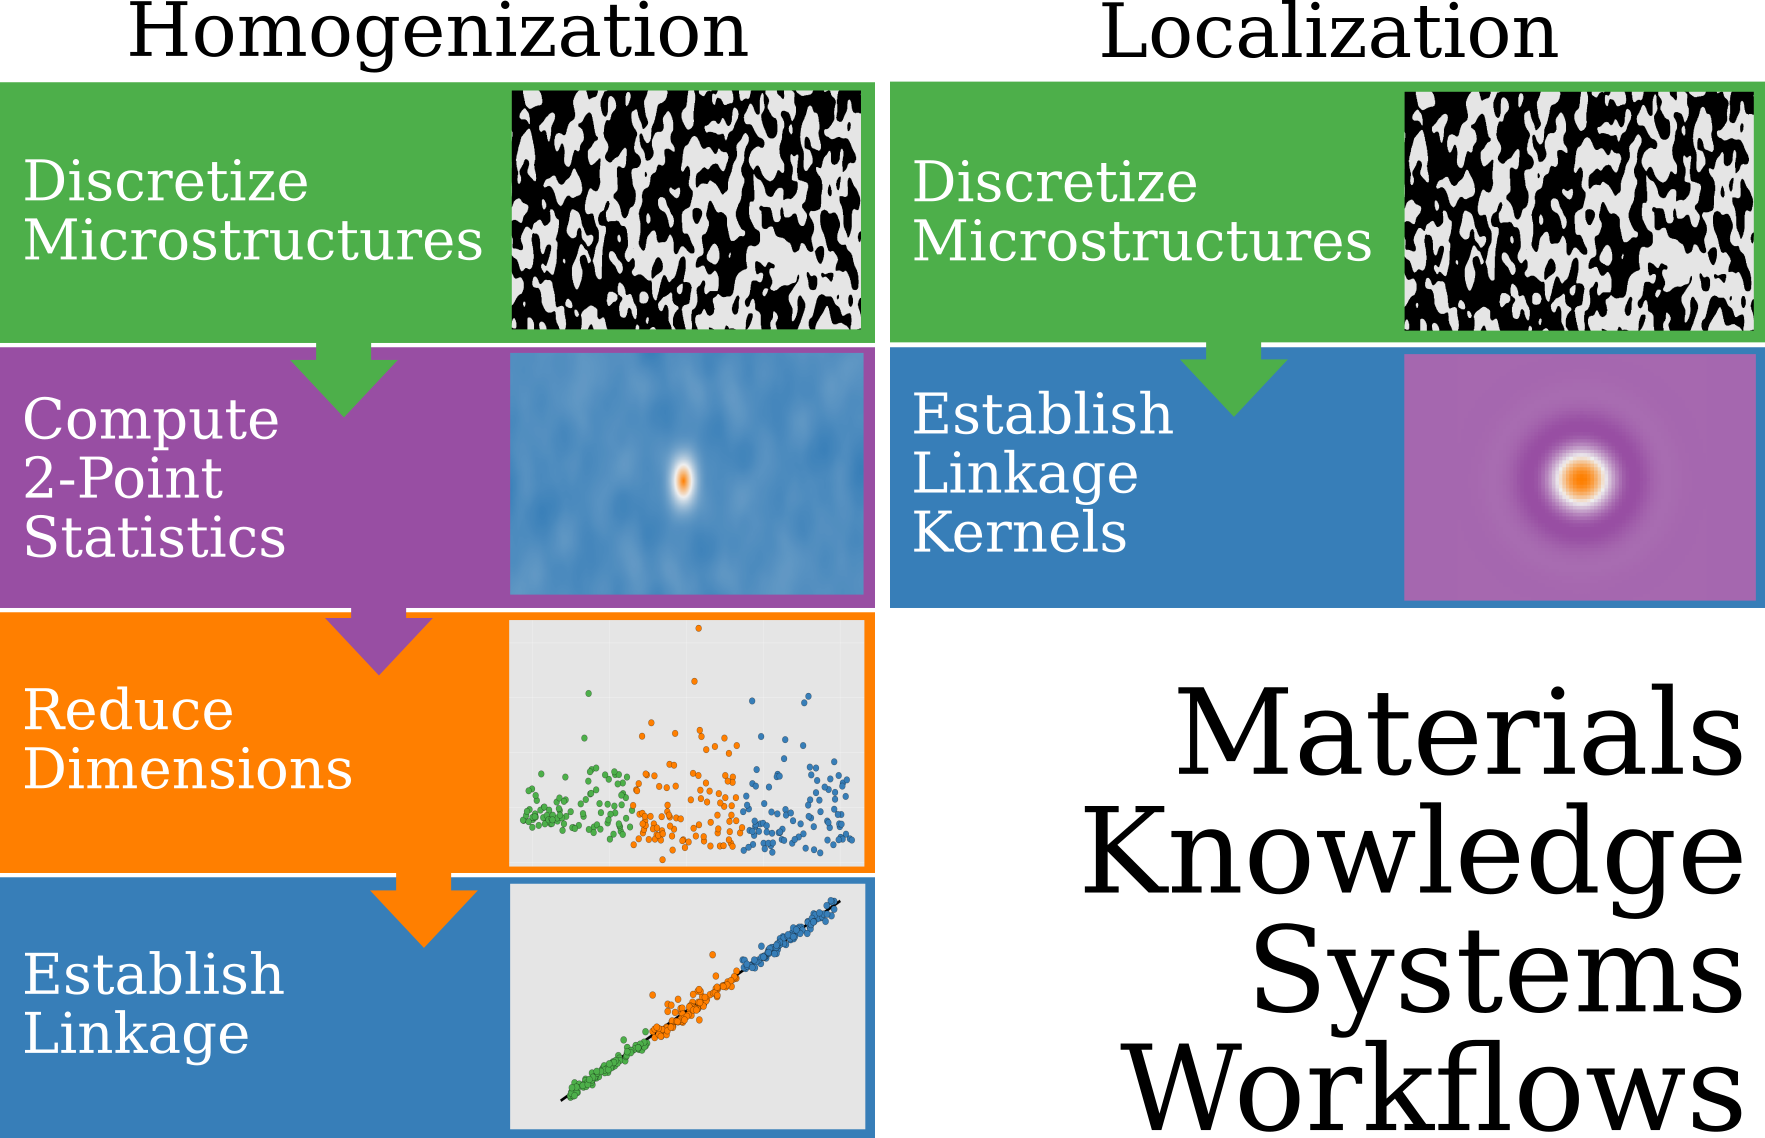
\includegraphics[scale=.22]{fig/mks_workflows.png}
  \label{fig:workflows}
\end{figure}


\section{Materials Knowledge Systems in Python}

PyMKS is an object-oriented numerical implementation of the MKS theory
developed in the literature~\cite{kalidindi2010novel}. It provides a
high-level, computationally efficient, framework to implement data
pipelines for classification, cataloging and quantifying materials
structures for PSP relationships. PyMKS is written in Python, a
natural choice for scientific computing due to its ubiquitous use
among the data science community as well as many other favorable
attributes~\cite{perez2011python}. PyMKS is licensed under the
permissive MIT license \cite{MIT} which allows for unrestricted
distribution in commercial and non-commercial systems.

\subsection{Core Functionality}


PyMKS consists of four main components including a set of tools to
compute 2-point statistics, tools for both homogenization and
localization linkages and tools for discretizing the microstructure. In
addition, PyMKS has modules for generating data sets using
conventional numerical simulations and a module for custom
visualization of microstructures. PyMKS builds on Scikit-learn's
pipelining methodology to create materials specific machine learning
models. This is a high level system for combining
multiple data and machine learning transformations into a single
customizable pipeline with only minimal required code. This approach
makes cross-validation and parameter searches simple to implement and
avoids the complicated book keeping issues associated with training,
testing and validating data pipelines in machine learning.

The starting point for an MKS homogenization analysis is to use
2-point statisics as outlined in Eq.~\ref{eq:stats} and provided in
PyMKS by the \texttt{MKSStructureAnalysis} object, which calculates
the objective low dimensional structure descriptors, $\mu_j[k]$. The
default dimensionality reduction technique is PCA, but any model that
uses the \texttt{transform\_fit} or a ``transformer'' object can be
substituted. After calculating the descriptors, the
\texttt{MKSHomogenizationModel} is used to create linkages between the
$\mu_j[k]$ and the effective material response, $p_j^{\text{eff}}$, as
indicated in Eq.~\ref{eq:hom}. The default machine learning algorithm
is a polynomial regression, but any estimator with the \texttt{fit}
and \texttt{predict} methods can be substituted to create the linkages
between $\mu_j[k]$ and $p_j^{\text{eff}}$.

The \texttt{MKSLocalizationModel} object provides the MKS localization
functionality. It calibrates the first order influence kernels
$\alpha[h; r]$ used to predict local materials responses, $p_j[s]$, as
outlined in Eq.~\ref{eq:series}. The calibration of the influence
kernels is achieved using a variety of linear regression techniques
described in numerous previous studies~\cite{landi2010multi,
kalidindi2010novel, yabansu2014calibrated, brough2016microstructure}.
The \texttt{MKSLocalizationModel} object uses \texttt{fit} and
\texttt{predict} methods to follow the standard interface for a
Scikit-learn estimator object.

To use either the homogenization or the localization models in PyMKS,
the microstructure first needs to be represented by a microstructure
function, $m_j\left[h, s\right]$. The \texttt{bases} module in PyMKS
contains four transformer objects for generating the
$m_j\left[h,s\right]$ using a varietly of discretization
methods~\cite{landi2010multi, kalidindi2010novel,
yabansu2014calibrated, al2012multi, kalidindi2011microstructure,
gupta2015structure, cceccen2014data, brough2016microstructure}.
These four objects can be thought of as materials specific
extension to the feature extraction
module in Scikit-learn. A \texttt{PrimitiveBasis} object uses
indicator (or hat) functions and is well suited for microstructures
that have discrete local states (e.g., distinct thermodynamic
phases). The \texttt{LegendreBasis} and \texttt{FourierBasis} objects
create spectral representations of microstucture functions defined on
nonperiodic and periodic continuous local state spaces,
respectively. For example, functions over a range of chemical
compositions can be described using \texttt{LegendreBasis}, while
functions over orientations in two-dimensional space can be described
using \texttt{FourierBasis}. Furthermore, \texttt{GSHBasis} creates
compact spectral representations for functions over lattice
orientation space (such as those needed to describe polycrystalline
microstructures)~\cite{ kalidindi2006spectral, shaffer2010building,
knezevic2010deformation, al2010spectral, duvvuru2007application,
li2003evolution, li2005texture, li2007processing, li2005processing,
creuziger2014crystallographic, sundararaghavan2008multi,
sundararaghavan2007linear}.

PyMKS contains modest data generation tools (in the \texttt{datasets}
module) that are used in both the PyMKS examples and the PyMKS test
suite. The \texttt{MicrostructureGenerator} object creates stochastic
microstructures using digital filters. This assists users in creating
PyMKS workflows even when data is unavailable. PyMKS has objects for
generating sample data from both a spinodal decomposition simulation
(using the \texttt{CahnHilliardSimulation} object) and a linear
elasticity simulation (using the \texttt{ElasticFESimulation}
object). PyMKS comes with custom functions for visualizing
microstructures in elegant ways (in the \texttt{tools} module). These
are used extensively in the PyMKS example notebooks to minimize
incidental code associated with visualization.

\subsection{Underlying Technologies}

PyMKS is built upon the highly optimized Python packages
NumPy~\cite{van2011numpy}, SciPy~\cite{jones2014scipy}, and
Scikit-learn~\cite{pedregosa2011scikit}. NumPy arrays are the primary
data structure used throughout PyMKS and provide the basic vector and
matrix manipulation operations. SciPy's signal processing and
numerical linear algebra functions are used to calibrate models and
generate synthetic data. PyMKS is highly integrated with Scikit-learn
and mimics its simple API in order to leverage from Scikit-learn's
data pipeling methodology for machine learning and data
transformations. In addition, PyMKS uses the Pytest framework to
automate execution of the test suite~\cite{pytest2016}.

Optional packages that can be used with PyMKS include Simple Finite
Elements in Python (SfePy)~\cite{cimrman2014sfepy}, the python wrapper
for the FFTW library (pyFFTW)~\cite{frigo1998fftw} and the plotting
package Matplotlib~\cite{hunter2007matplotlib}. SfePy is used to
simulate linear elasticity to create sample response field
data. PyFFTW is a hightly optimized Fast Fourier Transform library
that enhances the efficiency of PyMKS and enables parallel
computations in PyMKS. Matplotlib is used to generate custom
microstructure visualizations.

\subsection{Development Practices}

PyMKS leverages from existing tools, standards and web resources
wherever possible. In particular the developers are an open community
that use GitHub for issue tracking and release management
(see~\url{https://github.com/materialsinnovation/pymks}). Additionally
a Google group is used as a public forum to discuss the project
development, support and announcements
(see~\url{pymks-general@googlegroups.com}). The Travis CI continuous
integration tool is used to automate running the test suite for
branches of the code stored on GitHub. Code standards are maintained
by following the Python PEP8 standards and by reviewing code using
pull requests on GitHub. Detailed administrative guidelines are
outlined in the \texttt{ADMINISTRATA.md} document, and potential
developers are encouraged to follow them.

\section{Examples of Homogenization and Localization with PyMKS}

A demonstration of the MKS homogenization and localization
workflows as shown in Fig. \ref{fig:workflows}
are presented in this section using PyMKS. Additional workflow examples
can be found on the PyMKS website \url{pymks.org}.

\subsection{Prediction of Effective Stiffness with
Homogenization}\label{prediction-of-effective-stiffness-with-homogenization}

    \subsubsection{Generation of Calibration Data}\label{calibration-data-generation}

In this example the \texttt{MKSHomogenizationModel} is used to create a
structure-property linkage between a 2-phase composite material and
effective stiffness \(C_{xx}\).

Multiple classes of periodic microstructures and their effective elastic
stiffness values can be generated by importing the
\texttt{make\_elastic\_stiffness} function from \texttt{pymks.datasets}.

This function has several arguments. \texttt{n\_samples} is a list
indicating the number of microstructures for each class.
\texttt{grain\_size} and \texttt{volume\_fraction} are also lists that
specify the average grain features and mean volume fractions for each of
the microstructure classes. Variance in the volume fractions for each
class can be controlled using \texttt{percent\_variance} which specifies
a range of volume fractions centered about the mean values (i.e.
\texttt{volume\_fration} \(\pm\) \texttt{percent\_variance}).
\texttt{size} indicates the dimensions of all the microstructures.
\texttt{elastic\_modulus} and \texttt{poissons\_ratio} are used to
indicate the material properties for each of the phases. Lastly,
\texttt{seed} is used as the seed for the random number generator.

In this homogenization example, 50 samples from 16 different
microstructures classes with dimensions 21 x 21 and their effective
stiffness values were created totaling to 800 samples. Each of the 16
classes have different sized microstructure features and volume
fractions. The \texttt{make\_elastic\_stiffness} function returns the
microstructures \texttt{X} and their associated stiffness values
\texttt{y}.


\begin{_input}
from pymks.datasets import make_elastic_stiffness
import numpy as np

sample_size = 50
n_samples = [sample_size] * 16

grain_size = [(8, 8), (8, 6), (6, 8), (6, 6),
              (10, 4), (4, 10), (4, 4), (10, 10),
              (12, 2), (2, 12), (2, 2), (12, 12),
              (14, 1), (1, 14), (1, 1), (14, 14)]

volume_fraction = [(0.8, 0.2), (0.7, 0.3), (0.6, 0.4), (0.5, 0.5),
                   (0.2, 0.8), (0.3, 0.7), (0.4, 0.6), (0.5, 0.5),
                   (0.8, 0.2), (0.7, 0.3), (0.6, 0.4), (0.5, 0.5),
                   (0.2, 0.8), (0.3, 0.7), (0.4, 0.6), (0.5, 0.5)]

percent_variance = 0.15
elastic_modulus = (300, 200)
poissons_ratio = (0.28, 0.3)
size = (21, 21)
seed = 1

X, y = make_elastic_stiffness(n_samples=n_samples,
                              volume_fraction=volume_fraction,
                              grain_size=grain_size,  size=size,
                              percent_variance=percent_variance,
                              elastic_modulus=elastic_modulus,
                              poissons_ratio=poissons_ratio,
                              seed=seed)

\end{_input}

    An example microstructure from each of the 16 classes can be
visualized by importing \texttt{draw\_microstructures} function from
\texttt{pymks.tools}. The output from \texttt{draw\_microstructures}
can be found in Fig. \ref{fig:drawMicro}.


\begin{_input}
 from pymks.tools import draw_microstructures

X_examples = X[1::sample_size]
draw_microstructures(X_examples, figsize=(4, 4))

\end{_input}

\begin{figure}
    \centering
    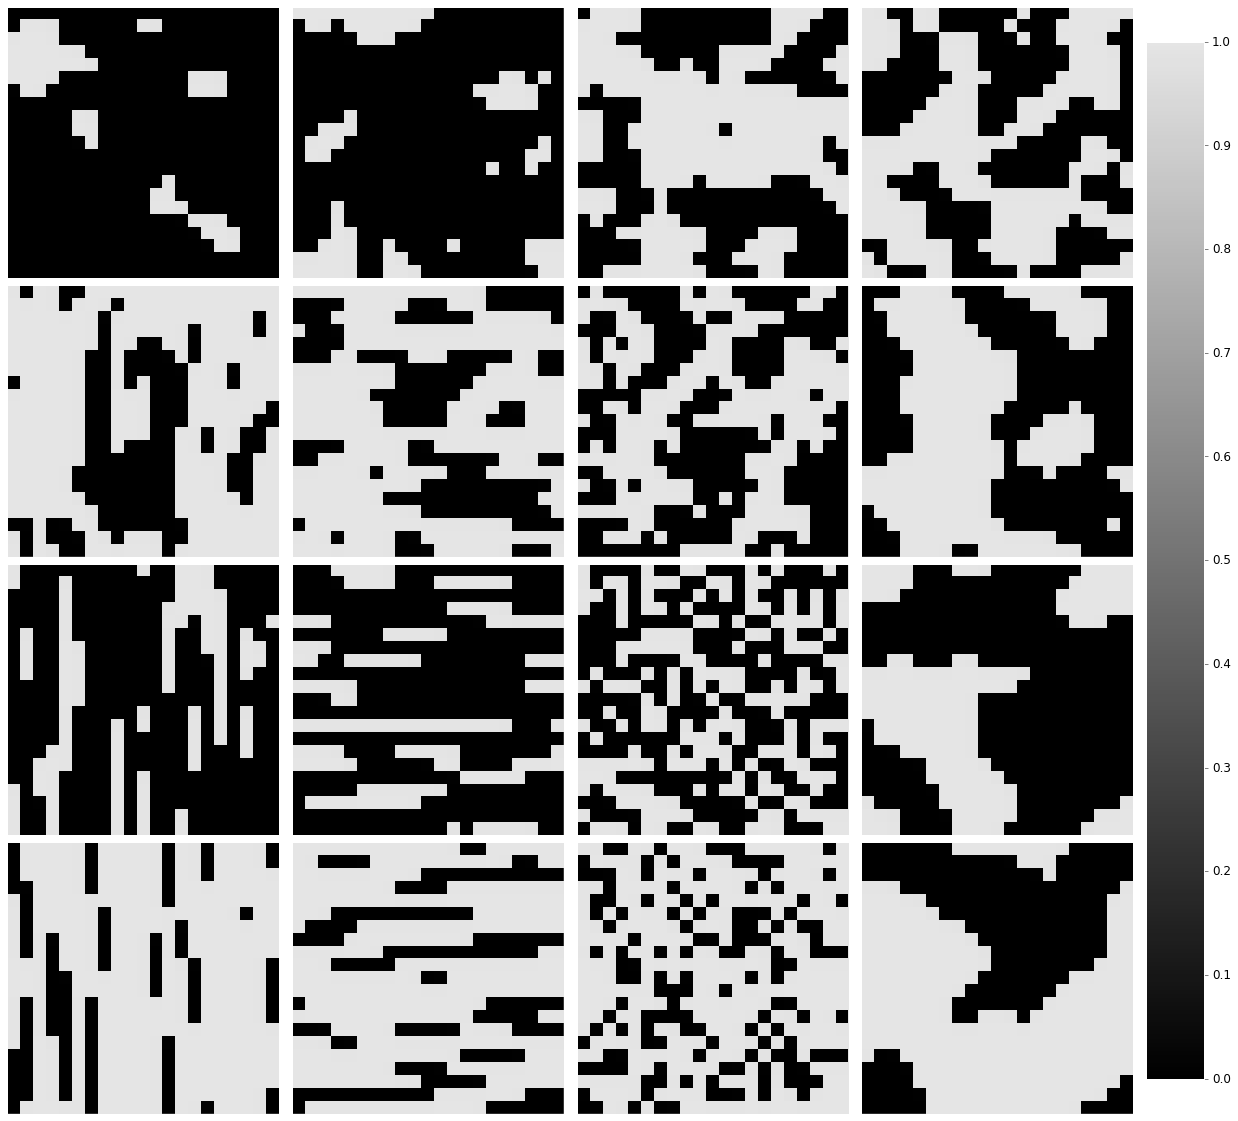
\includegraphics[scale=.28]{pymks_paper_homogenization_files/pymks_paper_homogenization_5_0.png}
    \caption{One sample from each of the 16 difference microstructure classes used for calibration of the homogenization model.}
    \label{fig:drawMicro}
\end{figure}

%     \begin{center}
%     \fimage{\adjustimage{max size={0.98\linewidth}{0.9\paperheight}}{pymks_paper_homogenization_files/pymks_paper_homogenization_5_0.png}}
%     \end{center}
%     { \hspace*{\fill} \\}
    \subsubsection{Calibration of Homogenization
Model}\label{calibration-of-homogenization-model}

Before an instance of the \texttt{MKSHomogenizationModel} can be made,
an instance of a basis class is needed to specify the discretization
method for the microstructure functions (see Fig. \ref{fig:workflows}).
For this particular example, there are only 2 discrete phases numerated
by 0 and 1. It has been shown that the primitive basis provides the most
compact representation of discrete phases \cite{niezgoda2013novel,niezgoda2011understanding,niezgoda2010optimized,
cecen2016versatile,cceccen2014data,landi2010multi,landi2010multi,
al2012multi}. In PyMKS the class
\texttt{PrimitiveBasis} from \texttt{pymks.bases} can be used with
\texttt{n\_states} equal to \texttt{2} and the \texttt{domain} equal to
\texttt{{[}0,\ 1{]}}.

The periodic axes as well as the set(s) of spatial correlations need to be specified in addition to the basis class for the
\texttt{MKSHomogenizationModel}. This is done using the arguments
\texttt{periodic\_axes} and \texttt{correlations} respectively . In
practice the set of spatial correlations are a hyper parameter of our
model that could be optimized, but for this example only the two
autocorrelations will be used.


\begin{_input}
from pymks import MKSHomogenizationModel
from pymks import PrimitiveBasis

prim_basis = PrimitiveBasis(n_states=2, domain=[0, 1])
model = MKSHomogenizationModel(basis=prim_basis,
                               periodic_axes=[0, 1],
                               correlations=[(0, 0), (1, 1)])
\end{_input}

The default pipeline used to create the homogenization linkage uses
PCA and polynomial regression objects for Scikit-learn. Using
\texttt{GridSearchCV} from Scikit-learn, cross validation is used on
the testing data to find the optimal number of principal components
and degree of polynomial (based on the R-squared values) within a
defined subspace for the hyper parameters for our model. A dictionary
\texttt{params\_to\_tune} defines the subspace. For this example
\texttt{n\_components} will be varied between 1 to 13 and
\texttt{degree} of the polynomial regression will be varied between 1
to 3. \texttt{StratifiedKFold} is used to ensure that microstructures
from each of the classes are used for each fold during cross
validation. The array \texttt{labels} is used to label each of the
classes.

\begin{_input}
from sklearn.cross_validation import StratifiedKFold
from sklearn.grid_search import GridSearchCV

flat_shape = (X.shape[0],) + (X[0].size,)
params_to_tune = {'degree': np.arange(1, 4),
                  'n_components': np.arange(1, 13)}
labels = np.repeat(np.arange(16), 50)
skf = StratifiedKFold(labels, n_folds=5)

fit_params = {'size': X[0].shape}
gs = GridSearchCV(
    model, params_to_tune, cv=skf,
    \usepackage{courier}fit_params=fit_params).fit(X.reshape(flat_shape), y)

\end{_input}

The results of our parameter grid search can be examined by either
printing or creating visualizations. The parameters and score of the
best estimator can be printed as shown below.

\begin{_input}
from __future__ import print_function

print('Order of Polynomial', gs.best_estimator_.degree)
print('Number of Components', gs.best_estimator_.n_components)
print('R-squared Value', gs.score(X, y))

\end{_input}
\begin{_output}
Order of Polynomial 2
Number of Components 11
R-squared Value 0.999960653331

\end{_output}


Two different visualizations of the results from \texttt{GridsearchCV}
with can be created using \texttt{draw\_gridscores\_matrix} and
\texttt{draw\_gridscores} from \texttt{pymks.tools}.

\texttt{draw\_gridscores\_matrix} provides a visualization of two
matrices for both the mean R-squared values and their standard
deviation. The output from \texttt{draw\_gridscores\_matrix} can be
found in Fig. \ref{fig:drawGridscoresMatrix}.


\begin{_input}
from pymks.tools import draw_gridscores_matrix

draw_gridscores_matrix(gs, ['n_components', 'degree'],
                       score_label='R-Squared',
                       param_labels=['Number of Components',
                                     'Order of Polynomial'])

\end{_input}



\begin{figure}
    \centering
    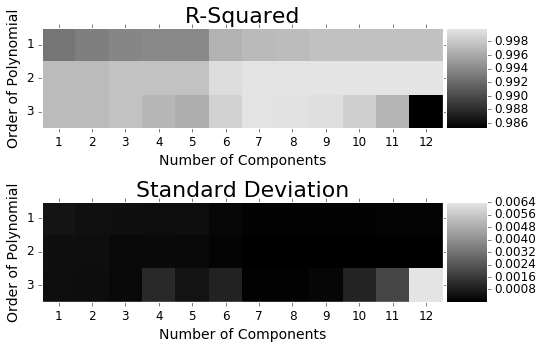
\includegraphics[scale=.64]{pymks_paper_homogenization_files/pymks_paper_homogenization_13_0.png}
    \caption{Mean R-Squared values and Standard deviation as a function of the order of the polynomial
    and the number of principal components.}
    \label{fig:drawGridscoresMatrix}
\end{figure}

    \texttt{draw\_gridscores} provides another view of the same information
with the mean values indicated by the points and the standard deviation
indication by the shared regions. The output from \texttt{draw\_gridscores}
can be found in Fig. \ref{fig:drawGridscores}.


\begin{_input}
from pymks.tools import draw_gridscores

gs_deg_1 = [x for x in gs.grid_scores_ \
            if x.parameters['degree'] == 1]
gs_deg_2 = [x for x in gs.grid_scores_ \
            if x.parameters['degree'] == 2]
gs_deg_3 = [x for x in gs.grid_scores_ \
            if x.parameters['degree'] == 3]

draw_gridscores([gs_deg_1,  gs_deg_2, gs_deg_3], 'n_components',
                data_labels=['1st Order',
                             '2nd Order', '3rd Order'],
                param_label='Number of Components',
                score_label='R-Squared')

\end{_input}

\begin{figure}
    \centering
    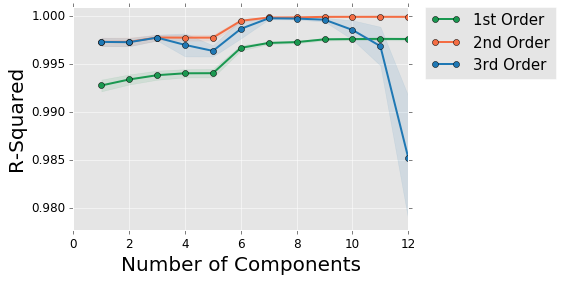
\includegraphics[scale=.625]{pymks_paper_homogenization_files/pymks_paper_homogenization_15_0.png}
    \caption{The mean R-Squared values indicated by the points and the standard deviation
indication by the shared regions as a function of the number of principal components for the first
three orders of a polynomial function.}
    \label{fig:drawGridscores}
\end{figure}

%     \begin{center}
% \fimage{\adjustimage{max size={0.98\linewidth}{0.9\paperheight}}{pymks_paper_homogenization_files/pymks_paper_homogenization_15_0.png}}
%     \end{center}
%     { \hspace*{\fill} \\}

    For the specified parameter range, the model with the highest R-squared
value was found to have a 2nd order polynomial with 11 principal
components. This model is calibrated using the entire training dataset and is
used for the rest of the example.

\begin{_input}
model = gs.best_estimator_

model.fit(X, y)
\end{_input}

    \subsubsection{Prediction of Effective Stiffness Values}\label{prediction-using-mkshomogenizationmodel}

In order to validate our model, additional data is generated using the
\texttt{make\_elastic\_stiffness} function again with the same
parameters with the exception of the number of samples and the seed used
for the random number generator. The function returns the new
microstructure \texttt{X\_new} and their effective stiffness values
\texttt{y\_new}.

\begin{_input}
test_sample_size = 10
n_samples = [test_sample_size] * 16

seed = 0

X_new, y_new = make_elastic_stiffness(
    n_samples=n_samples, size=size,
    grain_size=grain_size,
    volume_fraction=volume_fraction,
    percent_variance=percent_variance,
    elastic_modulus=elastic_modulus,
    poissons_ratio=poissons_ratio,
    seed=seed)
\end{_input}
    Effective stiffness values predicted by the model for the new
data are generated using the \texttt{predict} method.

\begin{_input}
y_pred = model.predict(X_new)
\end{_input}

    A visualization of the PC scores for both the
calibration and the validation data can be created using
\texttt{draw\_components\_scatter} from \texttt{pymks.tools}. The output from
\texttt{draw\_components\_scatter} can be found in Fig. \ref{fig:drawComponentsScatter}

Because both the validation and the calibration data were generated from
the \texttt{make\_elastic\_stiffness} function with the same parameters
both sets of data are different samples from the same distribution.
Similar visualizations can provide insights on differences between
different data sources.


\begin{_input}
from pymks.tools import draw_components_scatter

draw_components_scatter([model.reduced_fit_data[:, :2],
                         model.reduced_predict_data[:, :2]],
                        ['Training Data', 'Test Data'],
                        legend_outside=True)

\end{_input}

\begin{figure}
    \centering
    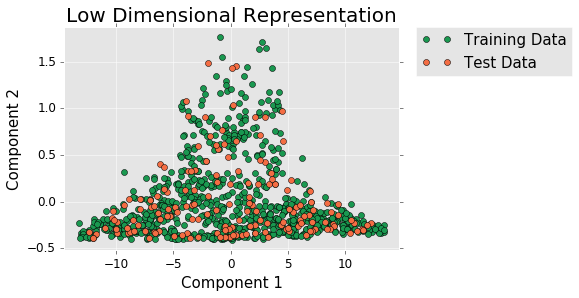
\includegraphics[scale=.61]{pymks_paper_homogenization_files/pymks_paper_homogenization_23_0.png}
    \caption{Low dimensional microstructure distributions ($\mu_j[k]$ from Eq. \ref{eq:struc}) for both the calibration and validation
    datasets.}
    \label{fig:drawComponentsScatter}
\end{figure}

%     \begin{center}
%     \fimage{\adjustimage{max size={0.98\linewidth}{0.9\paperheight}}{pymks_paper_homogenization_files/pymks_paper_homogenization_23_0.png}}
%     \end{center}
%     { \hspace*{\fill} \\}

    To evaluate our model's predictions, a goodness-of-fit plot can
be generated by importing \texttt{draw\_goodness\_of\_fit} from
\texttt{pymks.tools}. The results from \texttt{draw\_goodness\_of\_fit}
can be found in Fig. \ref{fig:drawGoodnessOfFit}. Additionally the R-squared
value for our predicted data can be printed.

\begin{_input}
from pymks.tools import draw_goodness_of_fit

fit_data = np.array([y, model.predict(X)])
pred_data = np.array([y_new, y_pred])
draw_goodness_of_fit(fit_data, pred_data,
                     ['Training Data', 'Test Data'])
\end{_input}



\begin{figure}
    \centering
    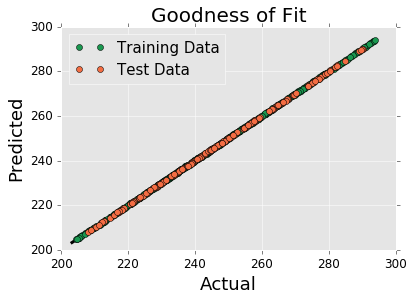
\includegraphics[scale=.85]{pymks_paper_homogenization_files/pymks_paper_homogenization_25_0.png}
    \caption{Goodness-of-Fit plot for effective stiffness $C_{xx}$ for the homogenization model.}
    \label{fig:drawGoodnessOfFit}
\end{figure}

%     \begin{center}
% \fimage{\adjustimage{max size={0.98\linewidth}{0.9\paperheight}}{pymks_paper_homogenization_files/pymks_paper_homogenization_25_0.png}}
%     \end{center}
%     { \hspace*{\fill} \\}

\begin{_input}
print('R-squared value', model.score(X_new, y_new))
\end{_input}
%     \begin{Verbatim}[commandchars=\\\{\}]
\begin{_output}
R-squared value 0.999949544961
\end{_output}
%     \end{Verbatim}

\subsection{Prediction of Local Strain Field with
Localization}\label{prediction-of-local-strain-field-with-localization}

\subsubsection{Generation of Calibration Data}\label{calibration-data-generation}

    In this example the \texttt{MKSLocalizationModel} is used to predict the
local strain field for a three phase microstructure with elastic moduli
values of 80 MPa, 100 MPa and 120 MPa; Poisson's ratio values all equal
to 0.3 and a macroscopic imposed strain equal to 0.02. The model is
calibrated using delta microstructures (analogous to using a unit
impulse response to find the kernel of a system in signal processing)
\cite{landi2010multi}. The the material parameters specified above
are used in a finite element simulation using the
\texttt{make\_elasticFEstrain\_delta} function from
\texttt{pymks.datasets}. The number of Poisson's ratio and elastic
moduli values indicates the number of phases.

\begin{_input}
from pymks.datasets import make_elastic_FE_strain_delta
import numpy as np

n = 21
n_phases = 3

elastic_modulus = (80, 100, 120)
poissons_ratio = (0.3, 0.3, 0.3)
macro_strain = 0.02
size = (n, n)

X_delta, strains_delta = make_elastic_FE_strain_delta(
    elastic_modulus=elastic_modulus,
    poissons_ratio=poissons_ratio,
    size=size, macro_strain=macro_strain)
\end{_input}
    Delta microstructures are composed of only two phases with the
center of the microstructure being a different phase from the rest. All
permutations of the delta microstructures and their associated strain
fields \(\varepsilon_{xx}\) are needed to calibrate the localization model.
A delta microstructure and it's strain field can be visualized using
\texttt{draw\_microstructure\_strain} from \texttt{pymks.tools}.
The output from \texttt{draw\_microstructure\_strain} can be found
in Fig. \ref{fig:drawMicroStrain}.

\begin{_input}
from pymks.tools import draw_microstructure_strain

draw_microstructure_strain(X_delta[0], strains_delta[0])
\end{_input}

\begin{figure}
    \centering
    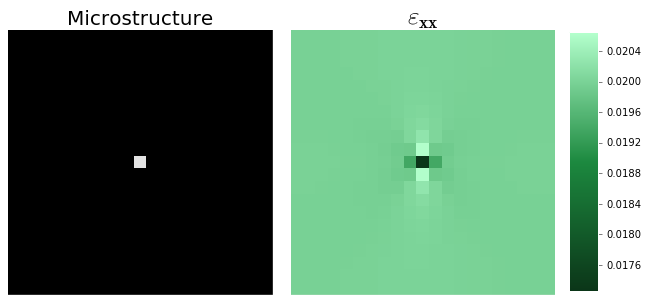
\includegraphics[scale=.54]{pymks_paper_localization_files/pymks_paper_localization_5_0.png}
    \caption{Delta microstructure (right) and its associated strain field (left). The delta
    microstructures and their local response fields are used to calibrated the localization model.}
    \label{fig:drawMicroStrain}
\end{figure}

%     \begin{center}
%     \fimage{\adjustimage{max size={0.98\linewidth}{0.9\paperheight}}{pymks_paper_localization_files/pymks_paper_localization_5_0.png}}
%     \end{center}
%     { \hspace*{\fill} \\}

    \subsubsection{Calibration of the Localization
Model}\label{calibration-of-the-localization-model}

    In order to make an instance of the \texttt{MKSLocalizationModel},
an instance of a basis class must first be created to specify the
discretization method for the microstructure function (see Fig.
\ref{fig:workflows}). For this particular example, there are 3 discrete
phases, therefore the \texttt{PrimitiveBasis} from \texttt{pymks.bases}
will be used. The phases are enumerated by 0, 1 and 2, therefore
we have three local states with a domain from 0 to 2. An instance of the
\texttt{PrimitiveBasis} with these parameters can be used to create an
instance of the \texttt{MKSLocalizationModel} as follows.

\begin{_input}
from pymks import MKSLocalizationModel
from pymks import PrimitiveBasis

p_basis =PrimitiveBasis(n_states=3, domain=[0, 2])
model = MKSLocalizationModel(basis=p_basis)
\end{_input}

    With the delta microstructures and their strain fields, the influence
kernels can be calibrated using the \texttt{fit} method.
A visualization of the influence kernels can be generated using the
\texttt{draw\_coeff} function from \texttt{pymks.tools}. The results
from \texttt{draw\_coeff} can be found in Fig. \ref{fig:drawCoeff}.

\begin{_input}
from pymks.tools import draw_coeff

model.fit(X_delta, strains_delta)
draw_coeff(model.coef_)
\end{_input}



\begin{figure}
    \centering
    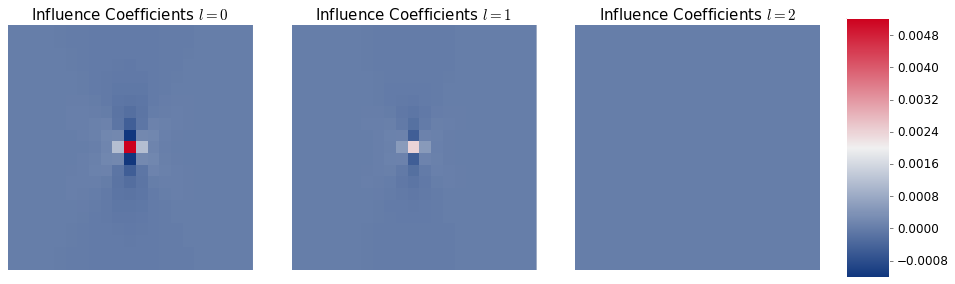
\includegraphics[scale=.37]{pymks_paper_localization_files/pymks_paper_localization_10_0.png}
    \caption{Calibrated influence kernels for the localization model.}
    \label{fig:drawCoeff}
\end{figure}

%     \begin{center}
%     \fimage{\adjustimage{max size={0.98\linewidth}{0.9\paperheight}}{pymks_paper_localization_files/pymks_paper_localization_10_0.png}}
%     \end{center}
%     { \hspace*{\fill} \\}
    \subsubsection{Prediction of the Strain Field for a Random
Microstructure}\label{prediction-of-the-strain-field-for-a-random-microstructure}

Model validation is done by comparing strain fields computed using a
finite element simulation and our localization model for the same random
microstructure. The \texttt{make\_elasticFEstrain\_random} function from
\texttt{pymks.datasets} generates a random microstructure and its
strain field results from finite element analysis. The output from
\texttt{make\_elasticFEstrain\_random} are visualized using
\texttt{draw\_microstructure\_strain} can be found in Fig.
\ref{fig:drawMicroStrainRandom}.


\begin{_input}
from pymks.datasets import make_elastic_FE_strain_random

np.random.seed(101)

X, strain = make_elastic_FE_strain_random(
    n_samples=1, elastic_modulus=elastic_modulus,
    poissons_ratio=poissons_ratio, size=size,
    macro_strain=macro_strain)

draw_microstructure_strain(X[0] , strain[0])

\end{_input}


\begin{figure}
    \centering
    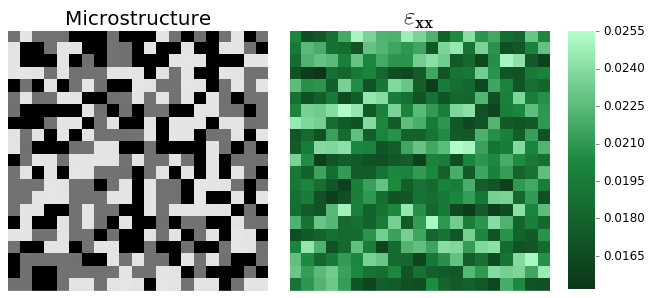
\includegraphics[scale=.54]{pymks_paper_localization_files/pymks_paper_localization_12_0.png}
    \caption{Random microstructure and its local strain field found using finite element analysis.}
    \label{fig:drawMicroStrainRandom}
\end{figure}

%     \begin{center}
%     \fimage{\adjustimage{max size={0.98\linewidth}{0.9\paperheight}}{pymks_paper_localization_files/pymks_paper_localization_12_0.png}}
%     \end{center}
%     { \hspace*{\fill} \\}
    The localization model predicts the strain field by passing the
random microstructure to the \texttt{predict} method. A visualization
of the two strain fields from both the localization model and finite element
analysis can be created using \texttt{draw\_strains\_compare} from
\texttt{pymks.tools}. The output from \texttt{draw\_strains\_compare}
can be found in Fig. \ref{fig:drawStrainCompare}.

\begin{_input}
from pymks.tools import draw_strains_compare

strain_pred = model.predict(X)
draw_strains_compare(strain[0], strain_pred[0])

\end{_input}

\begin{figure}
    \centering
    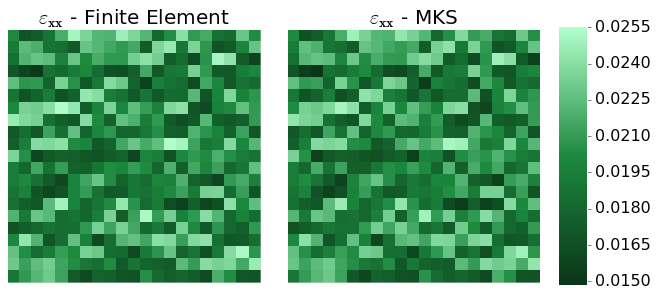
\includegraphics[scale=.535]{pymks_paper_localization_files/pymks_paper_localization_14_0.png}
    \caption{A comparison between the local strain field computed using finite element (left) and
    the prediction from the localization model (right).}
    \label{fig:drawStrainCompare}
\end{figure}



%     \begin{center}
%     \fimage{\adjustimage{max size={0.98\linewidth}{0.9\paperheight}}{pymks_paper_localization_files/pymks_paper_localization_14_0.png}}
%     \end{center}
%     { \hspace*{\fill} \\}

    These examples demonstrate the high level code that creates accurate and computationally efficient homogenization structure-property linkages using \texttt{MKSHomogenizationModel} and localization linkages using \texttt{MKSLocalizationModel} with PyMKS.

\section{Conclusion}

The MKS framework offers a practical and computationally efficient approach for distilling and disseminating the core knowledge gained from physics-based simulations and experiments using emerging concepts in modern data science. PyMKS is an open source project with a permissive license that provides simple high level APIs to access the MKS framework by implementing pipelines from Scikit-learn with customized objects for data from hierarchical materials. PyMKS has been launched with the aim to nucleate and grow an emergent community focused on establishing data-driven homogenization and localization Process-Structure-Property linkages for hierarchical materials.

%%%%%%%%%%%%%%%%%%%%%%%%%%%%%%%%%%%%%%%%%%%%%%
%%                                          %%
%% Backmatter begins here                   %%
%%                                          %%
%%%%%%%%%%%%%%%%%%%%%%%%%%%%%%%%%%%%%%%%%%%%%%

% \begin{backmatter}

% \section*{Competing interests}
%   The authors declare that they have no competing interests.

% \section*{Author's contributions}
%     Text for this section \ldots

\section*{Acknowledgements}

DBB and SRK acknowledge support from NSF-IGERT Award 1258425 and NIST 70NANB14H191.

%%%%%%%%%%%%%%%%%%%%%%%%%%%%%%%%%%%%%%%%%%%%%%%%%%%%%%%%%%%%%
%%                  The Bibliography                       %%
%%                                                         %%
%%  Bmc_mathpys.bst  will be used to                       %%
%%  create a .BBL file for submission.                     %%
%%  After submission of the .TEX file,                     %%
%%  you will be prompted to submit your .BBL file.         %%
%%                                                         %%
%%                                                         %%
%%  Note that the displayed Bibliography will not          %%
%%  necessarily be rendered by Latex exactly as specified  %%
%%  in the online Instructions for Authors.                %%
%%                                                         %%
%%%%%%%%%%%%%%%%%%%%%%%%%%%%%%%%%%%%%%%%%%%%%%%%%%%%%%%%%%%%%

% if your bibliography is in bibtex format, use those commands:
\bibliographystyle{bmc-mathphys} % Style BST file (bmc-mathphys, vancouver, spbasic).
\bibliography{bmc_article}      % Bibliography file (usually '*.bib' )
% for author-year bibliography (bmc-mathphys or spbasic)
% a) write to bib file (bmc-mathphys only)
% @settings{label, options="nameyear"}
% b) uncomment next line
%\nocite{label}

% or include bibliography directly:
% \begin{thebibliography}
% \bibitem{b1}
% \end{thebibliography}

%%%%%%%%%%%%%%%%%%%%%%%%%%%%%%%%%%%
%%                               %%
%% Figures                       %%
%%                               %%
%% NB: this is for captions and  %%
%% Titles. All graphics must be  %%
%% submitted separately and NOT  %%
%% included in the Tex document  %%
%%                               %%
%%%%%%%%%%%%%%%%%%%%%%%%%%%%%%%%%%%

%%
%% Do not use \listoffigures as most will included as separate files

% \section*{Figures}
%   \begin{figure}[h!]
%   \caption{\csentence{Sample figure title.}
%       A short description of the figure content
%       should go here.}
%       \end{figure}

% \begin{figure}[h!]
%   \caption{\csentence{Sample figure title.}
%       Figure legend text.}
%       \end{figure}

%%%%%%%%%%%%%%%%%%%%%%%%%%%%%%%%%%%
%%                               %%
%% Tables                        %%
%%                               %%
%%%%%%%%%%%%%%%%%%%%%%%%%%%%%%%%%%%

%% Use of \listoftables is discouraged.
%%
% \section*{Tables}
% \begin{table}[h!]
% \caption{Sample table title. This is where the description of the table should go.}
%       \begin{tabular}{cccc}
%         \hline
%           & B1  &B2   & B3\\ \hline
%         A1 & 0.1 & 0.2 & 0.3\\
%         A2 & ... & ..  & .\\
%         A3 & ..  & .   & .\\ \hline
%       \end{tabular}
% \end{table}

%%%%%%%%%%%%%%%%%%%%%%%%%%%%%%%%%%%
%%                               %%
%% Additional Files              %%
%%                               %%
%%%%%%%%%%%%%%%%%%%%%%%%%%%%%%%%%%%

% \section*{Additional Files}
%   \subsection*{Additional file 1 --- Sample additional file title}
%     Additional file descriptions text (including details of how to
%     view the file, if it is in a non-standard format or the file extension).  This might
%     refer to a multi-page table or a figure.

%   \subsection*{Additional file 2 --- Sample additional file title}
%     Additional file descriptions text.


% \end{backmatter}
\end{document}
